% Provenance (never printed): see sources/outline_sources.md (Year 2: Goldschmidt's
% classification; the chondritic Earth; core, mantle and crust compositions; trace
% elements and normalised diagrams). Curves from figdata/bachelor-2/geochem.py; exercise
% and problem values in the Book 4 scratch calculator calc/ch03.py.
\chapter{Elements in the Earth}\label{ch:b2:elements-in-the-earth}

A tonne of the rocks of the continents holds about one and a half milligrams of
gold. A tonne of the \omterm{def:b2:planet-formation-meteorites:chondrule}{carbonaceous chondrites} of the previous chapter, the most
primitive stones that fall from the sky, holds about a hundred times more. The
Earth was assembled from such material, so the gold is not missing from the
Earth: it is elsewhere. Combine the estimated compositions of the core and of
the silicate Earth with the mass of the core, and more than 99 per cent of the
Earth's gold turns out to sit in the core, where it sank with the iron early in
the Earth's history. Gold is one of a family of elements that follow metallic
iron; others follow sulfide, others the silicate rock, and others still escape
to the air. This chapter sorts the elements into these families, uses the
\omterm{def:b2:planet-formation-meteorites:chondrule}{chondrites} to reconstruct the composition of the whole Earth and to weigh its
core, describes the compositions of the mantle, the oceanic crust and the
continental crust, and introduces the \omterm{def:b2:elements-in-the-earth:trace}{trace elements} and the diagrams on which
geochemists read the history of a rock.
% ledger: rg03:ucc-trace, lodders:ci-table, mcd03:core, ms95:pm-trace, data:prem

\begin{recall}
The Earth has a metallic core, mostly iron, under a silicate mantle and a thin
crust; seismology gives the radius and the density of each layer, and the core
is 5 to 10 per cent less dense than pure iron would be at the same pressure and
temperature, which calls for light elements in it: silicon, sulfur, carbon,
oxygen and hydrogen are the candidates (Year 1 volume). The
electronegativity of an element measures how strongly its atoms attract the
electrons of a bond, and the radius of an ion depends on its charge and on the
number of its neighbours (chemistry books' Year 1 volume). A partition
coefficient is the ratio of the concentrations of a substance in two phases in
equilibrium (chemistry books' Year 1 volume). \omterm{def:b2:planet-formation-meteorites:chondrule}{Chondrites}, \omterm{def:b2:planet-formation-meteorites:chondrule}{carbonaceous
chondrites} and the \omterm{def:b2:planet-formation-meteorites:condensation}{condensation sequence} were introduced in
\cref{ch:b2:planet-formation-meteorites}.
\end{recall}
% ledger: badro:core

\section{Goldschmidt's classification}

When a chondritic body melts, its matter separates into immiscible liquids: a
dense metal of iron and nickel, a sulfide liquid if there is enough sulfur, and a
silicate melt, with a gas phase above. Each element distributes itself between
these phases according to its chemistry, and the same partition is seen in
smelting, where molten iron, a sulfide matte and a silicate slag separate in the
furnace.

\begin{definition}[Goldschmidt classification]
\label{def:b2:elements-in-the-earth:goldschmidt}
The \emph{Goldschmidt classification}\index{Goldschmidt classification} sorts
the elements by the phase they favour in a body that separates into metal,
sulfide, silicate and gas. A \emph{lithophile element}\index{lithophile element}
favours silicate and oxide; a \emph{siderophile element}\index{siderophile
element} favours metallic iron; a \emph{chalcophile
element}\index{chalcophile element} favours sulfide; an \emph{atmophile
element}\index{atmophile element} stays in the gas, as a gas or a volatile
compound.
\end{definition}

The classes follow the chemistry of bonding. \omterm{def:b2:elements-in-the-earth:goldschmidt}{Lithophile elements}, such as the
alkali and alkaline-earth metals, aluminium, titanium or the rare earths, give
up their electrons readily to oxygen, which is far more electronegative, and
form ionic bonds with it. \omterm{def:b2:elements-in-the-earth:goldschmidt}{Siderophile elements}, the platinum-group metals, gold,
nickel and cobalt, have electronegativities close to that of iron, bond weakly
with oxygen and dissolve in the metal. \omterm{def:b2:elements-in-the-earth:goldschmidt}{Chalcophile elements}, copper, zinc, lead,
silver and cadmium among them, form bonds with sulfur that are more covalent.
The \omterm{def:b2:elements-in-the-earth:goldschmidt}{atmophile elements} are the noble gases, nitrogen and hydrogen. Many
elements belong to two classes, depending on the conditions: iron itself is
siderophile in a metal-rich body and lithophile in the oxidised mantle, where it
sits in olivine and pyroxene; tungsten and molybdenum are siderophile in the
Earth, but much of them stayed in the mantle (figure below).

\begin{omfigure}
\centering
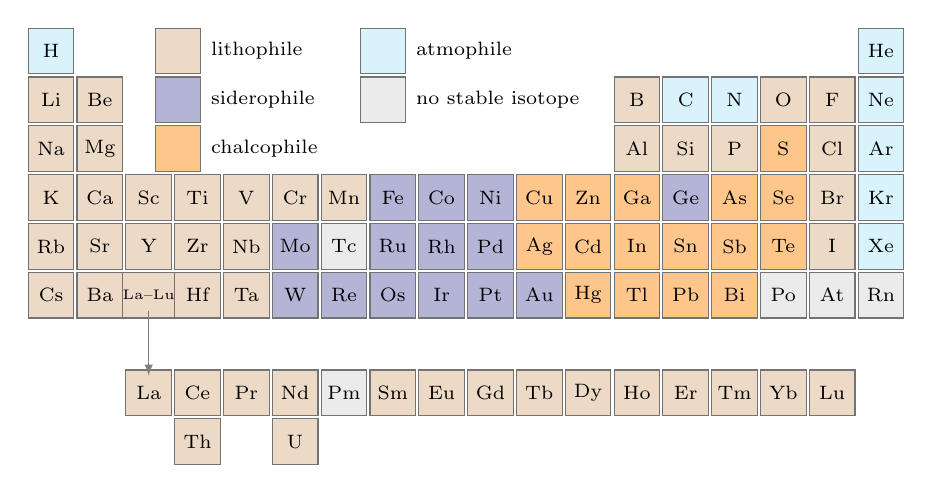
\begin{tikzpicture}[x=0.62cm, y=-0.62cm,
  lith/.style={fill=brown!30}, sid/.style={fill=blue!30!gray!45},
  chal/.style={fill=orange!45}, atm/.style={fill=cyan!15}, none/.style={fill=black!8},
  cell/.style={draw=black!55, minimum size=0.58cm, inner sep=0pt, font=\scriptsize}]
\foreach \s/\c/\r/\k in {H/1/1/atm, He/18/1/atm,
  Li/1/2/lith, Be/2/2/lith, B/13/2/lith, C/14/2/atm, N/15/2/atm, O/16/2/lith,
  F/17/2/lith, Ne/18/2/atm,
  Na/1/3/lith, Mg/2/3/lith, Al/13/3/lith, Si/14/3/lith, P/15/3/lith, S/16/3/chal,
  Cl/17/3/lith, Ar/18/3/atm,
  K/1/4/lith, Ca/2/4/lith, Sc/3/4/lith, Ti/4/4/lith, V/5/4/lith, Cr/6/4/lith,
  Mn/7/4/lith, Fe/8/4/sid, Co/9/4/sid, Ni/10/4/sid, Cu/11/4/chal, Zn/12/4/chal,
  Ga/13/4/chal, Ge/14/4/sid, As/15/4/chal, Se/16/4/chal, Br/17/4/lith, Kr/18/4/atm,
  Rb/1/5/lith, Sr/2/5/lith, Y/3/5/lith, Zr/4/5/lith, Nb/5/5/lith, Mo/6/5/sid,
  Tc/7/5/none, Ru/8/5/sid, Rh/9/5/sid, Pd/10/5/sid, Ag/11/5/chal, Cd/12/5/chal,
  In/13/5/chal, Sn/14/5/chal, Sb/15/5/chal, Te/16/5/chal, I/17/5/lith, Xe/18/5/atm,
  Cs/1/6/lith, Ba/2/6/lith, Hf/4/6/lith, Ta/5/6/lith, W/6/6/sid, Re/7/6/sid,
  Os/8/6/sid, Ir/9/6/sid, Pt/10/6/sid, Au/11/6/sid, Hg/12/6/chal, Tl/13/6/chal,
  Pb/14/6/chal, Bi/15/6/chal, Po/16/6/none, At/17/6/none, Rn/18/6/none,
  La/3/8/lith, Ce/4/8/lith, Pr/5/8/lith, Nd/6/8/lith, Pm/7/8/none, Sm/8/8/lith,
  Eu/9/8/lith, Gd/10/8/lith, Tb/11/8/lith, Dy/12/8/lith, Ho/13/8/lith,
  Er/14/8/lith, Tm/15/8/lith, Yb/16/8/lith, Lu/17/8/lith,
  Th/4/9/lith, U/6/9/lith}
  \node[cell, \k] at (\c,\r) {\s};
\node[cell, lith, minimum width=0.58cm] at (3,6) {\tiny La--Lu};
\draw[black!50, -latex] (3,6.32) -- (3,7.65);
% legend
\foreach \k/\t/\x/\y in {lith/lithophile/3.6/1, sid/siderophile/3.6/2,
  chal/chalcophile/3.6/3, atm/atmophile/7.8/1, none/{no stable isotope}/7.8/2}
  \node[cell, \k, label={[font=\scriptsize]east:\t}] at (\x,\y) {};
\end{tikzpicture}
\par\smallskip{\small The Goldschmidt classes of the stable elements and of thorium and uranium, whose long-lived isotopes survive from the Earth's birth, coloured by the class
that dominates in the Earth; elements of the rare earth row sit in the box
La--Lu. Several elements belong to two classes: iron, nickel and cobalt are also
lithophile in the oxidised mantle; carbon is also siderophile, phosphorus
siderophile in \omterm{def:b2:planet-formation-meteorites:fall-find}{meteorites}.}
\end{omfigure}

\section{The chondritic Earth}

No one can sample the Earth as a whole: the core is out of reach, and the
mantle reaches the surface only in pieces. The composition of the bulk Earth is
built instead from two pieces of evidence: the \omterm{def:b2:planet-formation-meteorites:fall-find}{meteorites}, which sample the
material from which the planets formed, and the rocks of the mantle and the
melts that come from it.

\begin{definition}[CI chondrite]\label{def:b2:elements-in-the-earth:ci}
A \emph{CI chondrite}\index{CI chondrite} is a member of the group of
\omterm{def:b2:planet-formation-meteorites:chondrule}{carbonaceous chondrites} named after the Ivuna \omterm{def:b2:planet-formation-meteorites:fall-find}{meteorite}: black, crumbly stones
made almost entirely of fine-grained matrix, rich in water-bearing minerals and
carbon, almost without \omterm{def:b2:planet-formation-meteorites:chondrule}{chondrules}. Apart from hydrogen, carbon, nitrogen, oxygen and the
noble gases, their composition is the closest of all known materials to that of
the Sun's photosphere; they are the reference composition of geochemistry.
\end{definition}

The group counts five \omterm{def:b2:planet-formation-meteorites:fall-find}{meteorites}, all of them falls: Alais (1806), Orgueil
(1864), Tonk (1911), Ivuna (1938) and Revelstoke (1965); Orgueil is the largest,
at fourteen kilograms. The composition adopted for the group is a weighted mean
of their analyses, element by element; the values used in this chapter are
quoted where they are needed.
% ledger: lodders:ci-table

\begin{definition}[Refractory and volatile elements]
\label{def:b2:elements-in-the-earth:volatility}
A \emph{refractory element}\index{refractory element} is one whose 50 per cent
\omterm{def:b2:planet-formation-meteorites:condensation}{condensation temperature} (\cref{ch:b2:planet-formation-meteorites}) lies above
those of magnesium, silicon and iron, \qtyrange{1310}{1340}{K} at
\qty{e-4}{bar}; a
\emph{volatile element}\index{volatile element} is one whose \omterm{def:b2:planet-formation-meteorites:condensation}{condensation
temperature} lies below them.
\end{definition}

The magnesium content serves as a yardstick. Magnesium is lithophile, condenses
with the bulk of the rock and does not enter the core, so the ratio of an element
to magnesium in the silicate Earth, divided by the same ratio in \omterm{def:b2:elements-in-the-earth:ci}{CI chondrites},
measures how much of that element the silicate Earth kept relative to a
chondritic starting material. The water, carbon and other volatile compounds that
\omterm{def:b2:elements-in-the-earth:ci}{CI chondrites} hold, which the Earth did not keep, cancel out of the ratio.

\begin{definition}[Bulk silicate Earth, primitive mantle]
\label{def:b2:elements-in-the-earth:bse}
The \emph{bulk silicate Earth}\index{bulk silicate Earth} is the Earth without
its core: mantle, crust, ocean and atmosphere taken together, as they would be if
mixed. The same composition is called the \emph{primitive mantle}\index{primitive
mantle}: the mantle as it was after the core formed and before any crust was
extracted from it.
\end{definition}

Estimates of the \omterm{def:b2:elements-in-the-earth:bse}{primitive mantle} rest on the mantle rocks that have lost the
least melt, peridotites brought up as xenoliths in lavas (photograph below) or
exposed in mountain belts, and on the assumption that the refractory \omterm{def:b2:elements-in-the-earth:goldschmidt}{lithophile
elements} stand in chondritic proportions to one another. One widely used result, with
magnesium 22.8, silicon 21.0 and iron 6.26 per cent by mass, is given in the
table of compositions further on.
% ledger: ms95:pm-trace, ms95:pm-oxides

\begin{omfigure}
\centering
\begin{minipage}{0.48\linewidth}
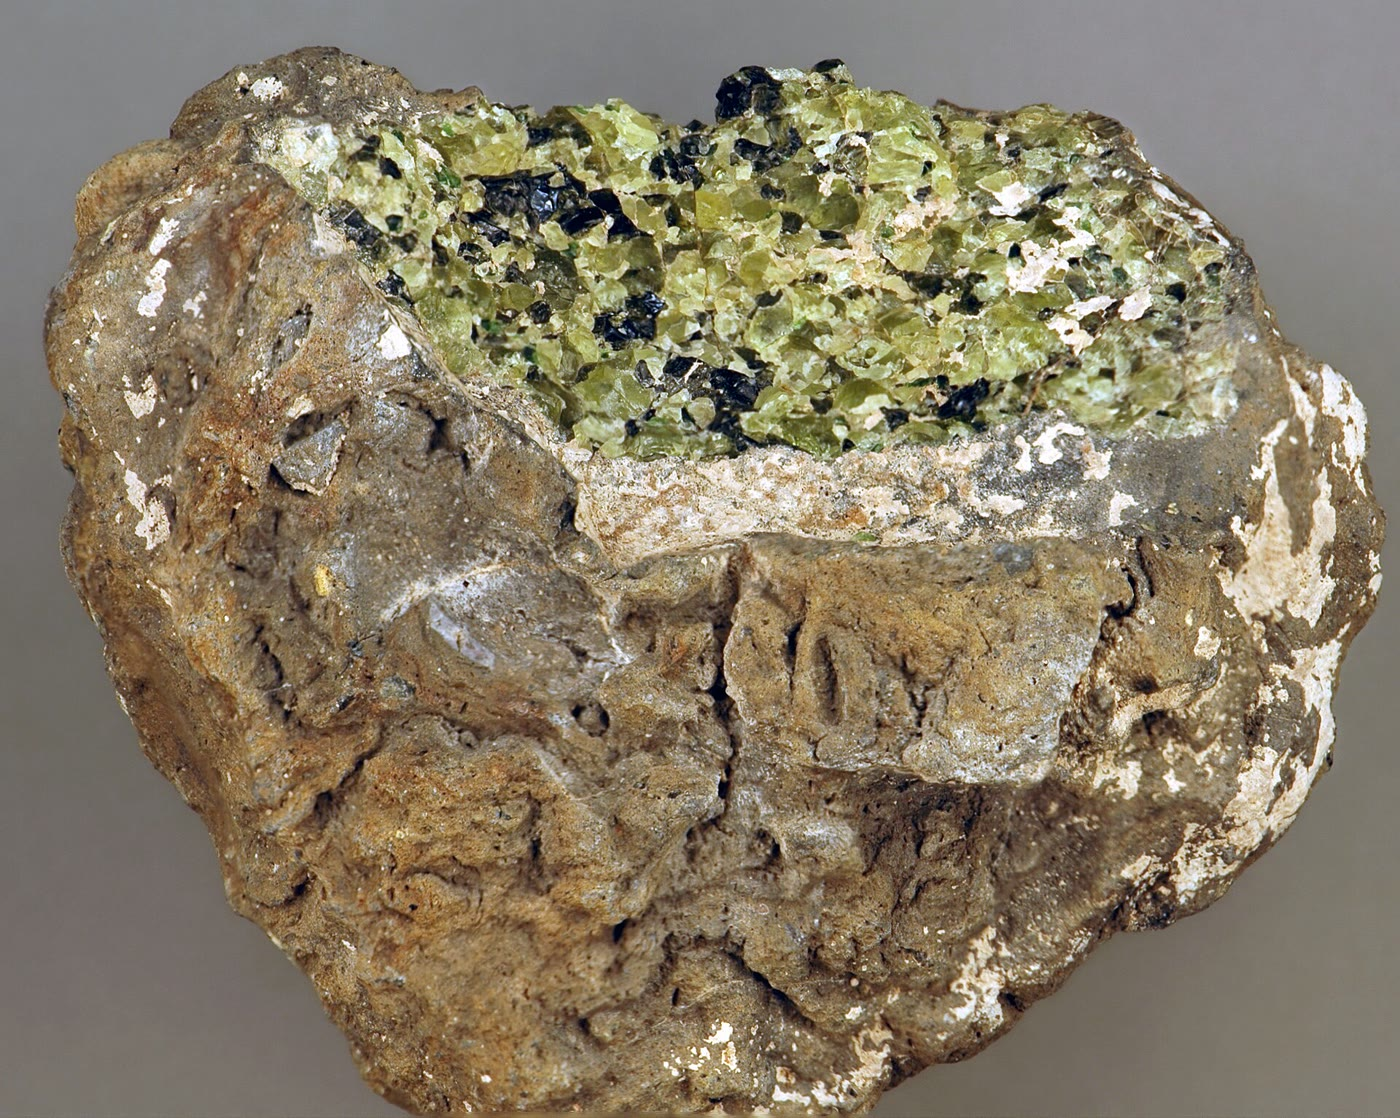
\includegraphics[width=\linewidth]{images/book4/b2-lherzolite-xenolith.jpg}
\end{minipage}\hfill
\begin{minipage}{0.48\linewidth}
{\small A nodule of mantle peridotite (lherzolite) in a basalt lava from
Kilbourne Hole, New Mexico, \qty{7.4}{cm} across at its widest: yellow-green
olivine with dark pyroxene. The lava tore it from the upper mantle and carried
it to the surface. James St.~John, CC BY 2.0.}
\end{minipage}
\end{omfigure}

The figure below compares this silicate Earth with \omterm{def:b2:elements-in-the-earth:ci}{CI chondrites}, element by
element, against the \omterm{def:b2:planet-formation-meteorites:condensation}{condensation temperature} of the previous chapter. It sorts
the elements in a way no other evidence can. The refractory \omterm{def:b2:elements-in-the-earth:goldschmidt}{lithophile
elements}, from zirconium and the rare earths down to strontium and barium, all
stand at the same level, within twenty per cent of one another: the silicate Earth
kept them all in their chondritic proportions. The volatile \omterm{def:b2:elements-in-the-earth:goldschmidt}{lithophile elements}
fall away with their \omterm{def:b2:planet-formation-meteorites:condensation}{condensation temperature}: about a fifth of the potassium
and sodium, a tenth of the rubidium, a hundredth of the chlorine and a few
thousandths of the bromine and iodine are there. The \omterm{def:b2:elements-in-the-earth:goldschmidt}{siderophile elements} lie far below every \omterm{def:b2:elements-in-the-earth:goldschmidt}{lithophile element}
of the same volatility: the silicate Earth holds a seventh of its share of
iron, a thirteenth of the nickel, and about three thousandths of the
platinum-group metals and gold. These went into the core. The \omterm{def:b2:elements-in-the-earth:goldschmidt}{chalcophile
elements}, most of them also volatile, are depleted on both counts.

\begin{omfigure}
\centering
\begin{tikzpicture}
\begin{axis}[omrecord, width=0.95\linewidth, height=8.2cm, ymode=log,
  xmin=500, xmax=1800, ymin=8e-4, ymax=3, x dir=reverse,
  xlabel={50 per cent condensation temperature at \qty{e-4}{bar} (K)},
  ylabel={$(X/\mathrm{Mg})_{\mathrm{BSE}}\,/\,(X/\mathrm{Mg})_{\mathrm{CI}}$},
  legend pos=south west, legend cell align=left, legend style={font=\scriptsize},
  tick label style={font=\scriptsize}, label style={font=\small},
  scaled x ticks=false, xticklabel style={/pgf/number format/1000 sep={}}]
\addplot[black!40, dashed, domain=500:1800, samples=2, forget plot] {1};
\addplot[only marks, mark=*, mark size=1.6pt, brown!70!black]
  table[x=T, y=ratio] {figdata/out/bachelor-2-geochem-volat-lith.dat};
\addlegendentry{lithophile}
\addplot[only marks, mark=square*, mark size=1.6pt, blue!60!black]
  table[x=T, y=ratio] {figdata/out/bachelor-2-geochem-volat-sid.dat};
\addlegendentry{siderophile}
\addplot[only marks, mark=triangle*, mark size=2pt, orange!80!black]
  table[x=T, y=ratio] {figdata/out/bachelor-2-geochem-volat-chal.dat};
\addlegendentry{chalcophile}
\node[font=\tiny, brown!50!black, anchor=south] at (axis cs:1600,1.35)
  {Zr, Hf, Al, Sc, Y, Th, U, Ti, Ca, Sr, Ba, rare earths};
\begin{scope}[font=\tiny, brown!50!black]
\node[anchor=west] at (axis cs:1328,1.0) {Mg};
\node[anchor=north] at (axis cs:1310,0.80) {Si};
\node[anchor=west] at (axis cs:1150,0.23) {Mn};
\node[anchor=south] at (axis cs:1142,0.47) {Li};
\node[anchor=south] at (axis cs:1010,0.195) {K};
\node[anchor=north] at (axis cs:958,0.22) {Na};
\node[anchor=north] at (axis cs:908,0.175) {B};
\node[anchor=north] at (axis cs:800,0.116) {Rb};
\node[anchor=south] at (axis cs:734,0.175) {F};
\node[anchor=west] at (axis cs:795,0.0477) {Cs};
\node[anchor=west] at (axis cs:944,0.0102) {Cl};
\node[anchor=north] at (axis cs:546,0.0061) {Br};
\node[anchor=south] at (axis cs:535,0.0088) {I};
\end{scope}
\begin{scope}[font=\tiny, blue!50!black]
\node[anchor=west] at (axis cs:1325,0.144) {Fe};
\node[anchor=east] at (axis cs:1364,0.0775) {Ni};
\node[anchor=west] at (axis cs:1342,0.088) {Co};
\node[anchor=west] at (axis cs:1780,0.137) {W};
\node[anchor=south] at (axis cs:1590,0.0206) {Mo};
\node[anchor=north] at (axis cs:883,0.0139) {Ge};
\node[anchor=north] at (axis cs:1500,0.0026) {Re, Os, Ir, Ru, Pt, Pd};
\node[anchor=north] at (axis cs:1060,0.0026) {Au};
\end{scope}
\begin{scope}[font=\tiny, orange!60!black]
\node[anchor=west] at (axis cs:1030,0.0993) {Cu};
\node[anchor=north] at (axis cs:996,0.0167) {Ag};
\node[anchor=south] at (axis cs:726,0.0746) {Zn};
\node[anchor=south] at (axis cs:704,0.0325) {Sn};
\node[anchor=east] at (axis cs:735,0.0246) {Pb};
\node[anchor=west] at (axis cs:648,0.0249) {Cd};
\node[anchor=east] at (axis cs:715,0.0022) {Te};
\node[anchor=north] at (axis cs:690,0.0016) {Se};
\node[anchor=west] at (axis cs:660,0.0019) {S};
\end{scope}
\end{axis}
\end{tikzpicture}
\par\smallskip{\small The silicate Earth compared with \omterm{def:b2:elements-in-the-earth:ci}{CI chondrites}: for each element $X$, the
ratio $X/\mathrm{Mg}$ in the \omterm{def:b2:elements-in-the-earth:bse}{bulk silicate Earth} divided by the same ratio in \omterm{def:b2:elements-in-the-earth:ci}{CI
chondrites}, against the 50 per cent \omterm{def:b2:planet-formation-meteorites:condensation}{condensation temperature} (hot on the left).
Refractory \omterm{def:b2:elements-in-the-earth:goldschmidt}{lithophile elements} are chondritic relative to one another; volatile
ones are depleted with falling \omterm{def:b2:planet-formation-meteorites:condensation}{condensation temperature}; siderophile and
\omterm{def:b2:elements-in-the-earth:goldschmidt}{chalcophile elements} are depleted far more. Data: McDonough and Sun (1995);
Lodders (2003).}
\end{omfigure}
% ledger: ms95:pm-trace, lodders:ci-table, lodders:tc-table, lodders:tc-more

The refractory \omterm{def:b2:elements-in-the-earth:goldschmidt}{lithophile elements} stand about 15 per cent above magnesium. The
two cannot both be exactly chondritic: either the Earth gained \omterm{def:b2:elements-in-the-earth:volatility}{refractory
elements}, or it lost a little magnesium, or the magnesium of the model is an
underestimate (\cref{exo:b2:elements-in-the-earth:12}). Silicon, at 0.83, falls further short of the
refractory level; part of the missing silicon may sit in the core (problem).

The \omterm{def:b2:elements-in-the-earth:goldschmidt}{siderophile elements} in the silicate Earth, combined with a chondritic bulk
Earth, weigh the core. Suppose the bulk Earth has the CI ratio $r_X = X/\mathrm{Mg}$
for a \omterm{def:b2:elements-in-the-earth:goldschmidt}{siderophile element} $X$, and the core holds the concentration $c_X$ of it
but no magnesium.

\begin{proposition}[Core mass fraction from a chondritic ratio]
\label{prop:b2:elements-in-the-earth:core}
Let $x$ be the mass fraction of the core, $C_X$ and $C_{\mathrm{Mg}}$ the
concentrations of $X$ and magnesium in the silicate Earth, and $c_X$ that of $X$ in
the core. If the Earth has the chondritic ratio $r_X$, then
\[
  \frac{x}{1-x} = \frac{r_X C_{\mathrm{Mg}} - C_X}{c_X}.
\]
\end{proposition}

\begin{proof}
A mass $M$ of Earth holds $(1-x)MC_X + xMc_X$ of $X$ and $(1-x)MC_{\mathrm{Mg}}$ of
magnesium. Their ratio is $r_X$:
$(1-x)C_X + xc_X = r_X(1-x)C_{\mathrm{Mg}}$. Dividing by $(1-x)c_X$ gives the
result.
\end{proof}

With iron, $r_{\mathrm{Fe}} = \num{182800}/\num{95870} = 1.907$ in \omterm{def:b2:elements-in-the-earth:ci}{CI chondrites},
22.8 per cent magnesium and 6.26 per cent iron in the silicate Earth, and 85.5 per
cent iron in a model core, the proposition gives $x/(1-x) = 0.435$, a core of 30
per cent of the Earth's mass. Seismology, integrating the density of the
reference Earth model, gives 32.5 per cent. The agreement to within a tenth
supports the picture of a chondritic Earth whose iron is mostly in the core; the
difference measures how far the Earth's iron-to-magnesium ratio departs from the
chondritic one (problem). The same balance tells where each element of the Earth is
(figure below): nearly all its platinum, iridium and gold, and most of its iron,
nickel and sulfur, are in the core.
% ledger: lodders:ci-table, ms95:pm-trace, mcd03:core, data:prem

\begin{omfigure}
\centering
\begin{tikzpicture}
\begin{axis}[omrecord, xbar, width=0.8\linewidth, height=6.4cm, bar width=5pt,
  xmin=0, xmax=100, ymin=0.4, ymax=14.6, y dir=reverse,
  ytick={1,...,14}, yticklabels from table={figdata/out/bachelor-2-geochem-budget.dat}{el},
  xlabel={share of the Earth's inventory held in the core (per cent)},
  tick label style={font=\scriptsize}, label style={font=\small},
  nodes near coords, nodes near coords align={horizontal},
  every node near coord/.append style={font=\tiny, /pgf/number format/fixed,
    /pgf/number format/precision=1}]
\addplot[fill=blue!35!gray!50, draw=black!60]
  table[x=share, y=idx] {figdata/out/bachelor-2-geochem-budget.dat};
\end{axis}
\end{tikzpicture}
\par\smallskip{\small Where the elements of the Earth are: the share of each element held in
the core, from a model core composition, the \omterm{def:b2:elements-in-the-earth:bse}{primitive mantle} and a core of 32.5
per cent of the Earth's mass. Data: McDonough (2003); McDonough and Sun (1995);
reference Earth model.}
\end{omfigure}
% ledger: mcd03:core, ms95:pm-trace, data:prem

\section{Mantle and crusts}

The silicate Earth has been divided since its formation into a mantle and two
kinds of crust. The oceanic crust is made by melting of the mantle beneath the
mid-ocean ridges; the continental crust by a long history of melting above
subduction zones, reworking and erosion (later chapters). Two reference melts
of the mantle anchor the discussion.

\begin{definition}[Mid-ocean ridge basalt, ocean island basalt]
\label{def:b2:elements-in-the-earth:morb-oib}
A \emph{mid-ocean ridge basalt}\index{mid-ocean ridge basalt} (MORB) is a basalt
erupted at a mid-ocean ridge, the rock of the top of the oceanic crust. An
\emph{ocean island basalt}\index{ocean island basalt} (OIB) is a basalt erupted
at an oceanic volcano away from plate boundaries, such as those of Hawaii,
commonly attributed to a mantle plume (Year 1 volume).
\end{definition}

The mean MORB in the table below is a global average built from 771 ridge
segments, each segment weighted by its length and its spreading rate, so that the
average represents the crust that the ridges produce. The OIB
column is a single rock: the basalt reference material BHVO-2, taken in 1995
from a lava that overflowed the Halemaumau crater of Kilauea, Hawaii, in 1919,
and analysed by many laboratories, so that most of its rare earths are known to
about one per cent. The upper continental crust is an average estimated from
surface rocks and sediments.
% ledger: gale13:allmorb, usgs:bhvo2-origin, usgs:bhvo2-major, rg14:crust

\begin{table}[h]
\centering
\small
\begin{tabular}{lrrrr}
\hline
oxide (wt\,\%) & \omterm{def:b2:elements-in-the-earth:bse}{primitive mantle} & MORB & OIB (BHVO-2) & upper cont.\ crust\\
\hline
\ce{SiO2} & 45.0 & 50.47 & 49.60 & 66.6\\
\ce{TiO2} & 0.201 & 1.68 & 2.731 & 0.64\\
\ce{Al2O3} & 4.45 & 14.70 & 13.44 & 15.4\\
FeO (total) & 8.05 & 10.43 & 11.15 & 5.04\\
MnO & 0.135 & 0.184 & 0.1690 & 0.10\\
MgO & 37.8 & 7.58 & 7.257 & 2.48\\
CaO & 3.55 & 11.39 & 11.40 & 3.59\\
\ce{Na2O} & 0.36 & 2.79 & 2.219 & 3.27\\
\ce{K2O} & 0.029 & 0.160 & 0.5130 & 2.80\\
\ce{P2O5} & 0.021 & 0.184 & 0.2685 & 0.15\\
\hline
\end{tabular}
\caption{Major-element compositions of four reservoirs. BHVO-2 gives its iron as
\ce{Fe2O3} (12.39 per cent), here converted to FeO. Data: McDonough and Sun
(1995); Gale and others (2013); USGS information sheet for BHVO-2; Rudnick and
Gao (2014).}
\label{tab:b2:elements-in-the-earth:majors}
\end{table}
% ledger: ms95:pm-oxides, gale13:allmorb, usgs:bhvo2-major, rg14:crust

Read across, the table tells the story of melting. The mantle is a magnesium-rich
peridotite, nearly 38 per cent MgO and less than 5 per cent of \ce{Al2O3} and CaO.
Its melts, the basalts, hold five times less magnesium and three times more
calcium and aluminium: the elements that enter the melt readily leave the mantle
first. Potassium, sodium and titanium are richer still in the melts compared
with the mantle, and potassium is richest of all in the continental crust,
nearly a hundred times its concentration in the \omterm{def:b2:elements-in-the-earth:bse}{primitive mantle}. Silicon rises
from the mantle to the basalts only a little, and much more in the continental
crust, whose average is close to that of a granodiorite.

\section{Trace elements}

Ten oxides make up more than 99 per cent of each rock of the table above. The remaining elements,
present at parts per million, follow the same processes as the major ones, but
they are much more sensitive to them.

\begin{definition}[Trace element]\label{def:b2:elements-in-the-earth:trace}
A \emph{trace element}\index{trace element} of a rock is an element whose
concentration is conventionally below 0.1 per cent by mass (\qty{1000}{ppm}).
Trace elements seldom form minerals of their own; they substitute for major
elements in the sites of the crystal lattices.
\end{definition}

A \omterm{def:b2:elements-in-the-earth:trace}{trace element} is so dilute that its own concentration does not change the
crystals or the melt: its distribution between them is then a simple ratio,
independent of its concentration over a wide range.

\begin{definition}[Mineral--melt partition coefficient; compatible and
incompatible elements]\label{def:b2:elements-in-the-earth:partition}
The \emph{mineral--melt partition coefficient}\index{mineral--melt partition
coefficient} of an element in a mineral is the ratio of its concentrations in the
mineral and in a silicate melt in equilibrium with it,
$D = C_{\mathrm{mineral}}/C_{\mathrm{melt}}$. For a rock of several minerals of
mass fractions $x_i$, the \emph{bulk partition coefficient} is
$\bar D = C_{\mathrm{rock}}/C_{\mathrm{melt}}$. An element is a
\emph{compatible element}\index{compatible element} in a rock if $\bar D > 1$,
an \emph{incompatible element}\index{incompatible element} if $\bar D < 1$.
\end{definition}

\begin{proposition}[Bulk partition coefficient]
\label{prop:b2:elements-in-the-earth:bulk-d}
If each mineral of the rock is in equilibrium with the same melt, the bulk
partition coefficient is the average of the mineral coefficients weighted by
the mass fractions: $\bar D = \sum_i x_i D_i$.
\end{proposition}

\begin{proof}
The rock holds $C_{\mathrm{rock}} = \sum_i x_i C_i$, and each mineral
$C_i = D_i C_{\mathrm{melt}}$. Dividing by $C_{\mathrm{melt}}$ gives the result.
\end{proof}

Whether an ion fits a site depends on its radius and its charge. An ion close in
radius and charge to the major ion of a site, such as \ce{Ni^2+} for \ce{Mg^2+} in
olivine, enters easily and is compatible. An ion much larger, such as
\ce{Rb+} or \ce{Ba^2+}, or more highly charged, such as \ce{Zr^4+} or
\ce{Nb^5+}, strains the lattice and is rejected into the melt: it is
incompatible in the minerals of the mantle. Two groups of \omterm{def:b2:elements-in-the-earth:partition}{incompatible elements}
behave differently later on, when water is involved.

\begin{definition}[Large-ion lithophile and high-field-strength elements]
\label{def:b2:elements-in-the-earth:lile-hfse}
The \emph{large-ion lithophile elements}\index{large-ion lithophile element}
(LILE) are \omterm{def:b2:elements-in-the-earth:partition}{incompatible elements} with large ions of low charge, $+1$ or $+2$:
potassium, rubidium, caesium, strontium, barium. The
\emph{high-field-strength elements}\index{high-field-strength element} (HFSE)
are \omterm{def:b2:elements-in-the-earth:partition}{incompatible elements} with small, highly charged ions, $+4$ or $+5$:
zirconium, hafnium, niobium, tantalum, titanium.
\end{definition}

The LILE dissolve easily in water-rich fluids, the HFSE hardly at all. A rock
altered by water or a melt that inherited fluids, as above subduction zones,
therefore carries LILE with little HFSE.

\begin{definition}[Rare earth elements]\label{def:b2:elements-in-the-earth:ree}
The \emph{rare earth elements}\index{rare earth element} (REE) are the fifteen
lanthanides, from lanthanum to lutetium; promethium has no stable isotope. All
are lithophile and refractory, nearly all trivalent, and their ionic radius
shrinks steadily from lanthanum to lutetium; europium can also be divalent in
reduced melts.
\end{definition}

Because the rare earths differ smoothly in radius and nothing else, they
fractionate smoothly: the light ones, lanthanum to samarium, are the least
compatible; the heavy ones, gadolinium to lutetium, fit better into some
minerals, above all garnet (figure below). In a rock with garnet, the heavy rare
earths become compatible: a melt of such a rock is rich in light rare earths and
poor in heavy ones.

\begin{omfigure}
\centering
\begin{tikzpicture}
\begin{axis}[omrecord, width=0.78\linewidth, height=6.4cm, ymode=log,
  xmin=0.6, xmax=9.4, ymin=5e-4, ymax=20,
  xtick={1,...,9}, xticklabels from table={figdata/out/bachelor-2-geochem-dvals.dat}{el},
  ylabel={partition coefficient $D$}, legend pos=south east,
  legend cell align=left, legend style={font=\scriptsize},
  tick label style={font=\scriptsize}, label style={font=\small}]
\addplot[black!40, dashed, domain=0.6:9.4, samples=2, forget plot] {1};
\addplot[thick, green!45!black, mark=*] table[x=idx, y=cpx] {figdata/out/bachelor-2-geochem-dvals.dat};
\addlegendentry{clinopyroxene}
\addplot[thick, red!70!black, mark=square*] table[x=idx, y=gar] {figdata/out/bachelor-2-geochem-dvals.dat};
\addlegendentry{garnet}
\addplot[thick, olive!70!black, mark=triangle*] table[x=idx, y=ol] {figdata/out/bachelor-2-geochem-dvals.dat};
\addlegendentry{olivine + orthopyroxene + spinel}
\addplot[very thick, black, mark=diamond*] table[x=idx, y=bulk] {figdata/out/bachelor-2-geochem-dvals.dat};
\addlegendentry{bulk rock (65/18/17 per cent)}
\node[font=\scriptsize, anchor=south west] at (axis cs:0.7,1) {compatible};
\node[font=\scriptsize, anchor=north west] at (axis cs:0.7,1) {incompatible};
\end{axis}
\end{tikzpicture}
\par\smallskip{\small \omterm{def:b2:elements-in-the-earth:partition}{Mineral--melt partition coefficients} of the rare earths for
clinopyroxene, garnet and a mix of olivine, orthopyroxene and spinel, and the
bulk coefficient of a garnet pyroxenite of 65 per cent clinopyroxene, 18 per
cent garnet and 17 per cent of the other minerals (Proposition above). Garnet
makes the heavy rare earths compatible. Data: Budahn (1991).}
\end{omfigure}
% ledger: budahn91:d-ree, budahn91:modes

\section{Normalised diagrams}

The abundances of neighbouring elements differ by large factors because of the
nuclear history of matter: elements of even atomic number are more abundant than
their odd neighbours, as the CI column of the rare earths shows (lanthanum 0.232,
cerium 0.621, praseodymium 0.0928 ppm). Plotted raw, a rock's rare earths form a
saw-tooth that hides its geological history. Dividing by a reference removes it.
% ledger: lodders:ci-table

\begin{definition}[Normalised diagram]\label{def:b2:elements-in-the-earth:normalised}
A \emph{normalised diagram}\index{normalised diagram} plots, for a series of
elements in a fixed order, the concentration in a sample divided by that in a
reference, $X_N = C_X/C_X^{\mathrm{ref}}$, on a logarithmic scale. The rare earths
are normalised to \omterm{def:b2:elements-in-the-earth:ci}{CI chondrites} in the order of atomic number; a longer set of
\omterm{def:b2:elements-in-the-earth:partition}{incompatible elements}, often called a spider diagram, is normalised to the
\omterm{def:b2:elements-in-the-earth:bse}{primitive mantle} and ordered by decreasing incompatibility in mantle melting.
\end{definition}

A sample with the same proportions as the reference plots as a horizontal line;
its height gives the enrichment. A slope shows a fractionation between light and
heavy elements, measured by a ratio such as $(\mathrm{La}/\mathrm{Yb})_N$. A
single element off the line is an anomaly.

\begin{proposition}[Europium anomaly]\label{prop:b2:elements-in-the-earth:normalised}
On a \omterm{def:b2:elements-in-the-earth:normalised}{normalised diagram} where the pattern is a straight line in
$\log X_N$ between samarium and gadolinium, the value expected for europium, which
lies midway, is $\mathrm{Eu}^* = \sqrt{\mathrm{Sm}_N\,\mathrm{Gd}_N}$. The
\emph{europium anomaly}\index{europium anomaly} is
$\mathrm{Eu}/\mathrm{Eu}^* = \mathrm{Eu}_N/\sqrt{\mathrm{Sm}_N\,\mathrm{Gd}_N}$:
below 1 it is negative, above 1 positive.
\end{proposition}

\begin{proof}
Samarium, europium and gadolinium are consecutive at equal steps along the axis.
A straight line in $\log X_N$ takes at the middle point the mean of the end values:
$\log \mathrm{Eu}^* = \tfrac12(\log \mathrm{Sm}_N + \log \mathrm{Gd}_N)$, the
logarithm of the geometric mean.
\end{proof}

Europium is the one rare earth that can be divalent. \ce{Eu^2+} has nearly the
radius of \ce{Ca^2+} and \ce{Sr^2+}, so plagioclase feldspar takes it in where it
rejects the trivalent rare earths. A melt from which plagioclase has crystallised
has a negative anomaly; the plagioclase-rich rock left behind, a positive one.

\begin{omfigure}
\centering
\begin{tikzpicture}
\begin{axis}[omrecord, width=0.8\linewidth, height=6.4cm, ymode=log,
  xmin=0.6, xmax=13.4, ymin=5, ymax=250,
  xtick={1,...,13}, xticklabels from table={figdata/out/bachelor-2-geochem-ree.dat}{el},
  ylabel={sample / CI chondrite}, legend pos=north east, legend cell align=left,
  legend style={font=\scriptsize}, tick label style={font=\scriptsize},
  label style={font=\small}]
\addplot[thick, blue!70!black, mark=*] table[x=idx, y=morb] {figdata/out/bachelor-2-geochem-ree.dat};
\addlegendentry{mean MORB}
\addplot[thick, red!70!black, mark=square*] table[x=idx, y=oib] {figdata/out/bachelor-2-geochem-ree.dat};
\addlegendentry{OIB (BHVO-2, Hawaii)}
\addplot[thick, brown!70!black, mark=triangle*] table[x=idx, y=ucc] {figdata/out/bachelor-2-geochem-ree.dat};
\addlegendentry{upper continental crust}
\end{axis}
\end{tikzpicture}
\par\smallskip{\small Rare earth patterns normalised to \omterm{def:b2:elements-in-the-earth:ci}{CI chondrites} (thulium left out, for
want of a MORB value). The mean MORB is flat, slightly poorer in the light rare
earths; the Hawaiian basalt is enriched in them; the upper crust is strongly
enriched in them, with a negative \omterm{prop:b2:elements-in-the-earth:normalised}{europium anomaly}. Data: Gale and others
(2013); USGS BHVO-2 sheet; Rudnick and Gao; Lodders (2003).}
\end{omfigure}
% ledger: gale13:allmorb, usgs:bhvo2-trace, rg03:ucc-trace, lodders:ci-table

The three patterns of the figure above read as three histories. The mean MORB
lies about 25 times above \omterm{def:b2:planet-formation-meteorites:chondrule}{chondrite}, nearly flat, with $(\mathrm{La}/\mathrm{Sm})_N
= 0.85$: its mantle source had already lost some of its most \omterm{def:b2:elements-in-the-earth:partition}{incompatible elements}
to earlier melts, the continental crust among them. The Hawaiian basalt is
enriched in the light rare earths, $(\mathrm{La}/\mathrm{Yb})_N = 5.4$, and its
heavy rare earths are lower than those of MORB: it came from a smaller degree of
melting, in which garnet was left behind holding the heavy ones. The upper
continental crust is enriched more than a hundred times in lanthanum, with
$(\mathrm{La}/\mathrm{Yb})_N = 10.9$ and $\mathrm{Eu}/\mathrm{Eu}^* = 0.72$: it is
the product of repeated melting, and its europium deficit is consistent with
plagioclase left behind in the deep crust.

\begin{omfigure}
\centering
\begin{tikzpicture}
\begin{axis}[omrecord, width=\linewidth, height=6.6cm, ymode=log,
  xmin=0.5, xmax=27.5, ymin=1, ymax=400,
  xtick={1,...,27}, xticklabels from table={figdata/out/bachelor-2-geochem-spider.dat}{el},
  ylabel={sample / primitive mantle}, legend pos=north east, legend cell align=left,
  legend style={font=\scriptsize}, tick label style={font=\scriptsize},
  label style={font=\small}]
\addplot[thick, blue!70!black, mark=*, mark size=1.4pt] table[x=idx, y=morb] {figdata/out/bachelor-2-geochem-spider.dat};
\addlegendentry{mean MORB}
\addplot[thick, red!70!black, mark=square*, mark size=1.4pt] table[x=idx, y=oib] {figdata/out/bachelor-2-geochem-spider.dat};
\addlegendentry{OIB (BHVO-2)}
\addplot[thick, brown!70!black, mark=triangle*, mark size=1.6pt] table[x=idx, y=ucc] {figdata/out/bachelor-2-geochem-spider.dat};
\addlegendentry{upper continental crust}
\end{axis}
\end{tikzpicture}
\par\smallskip{\small \omterm{def:b2:elements-in-the-earth:partition}{Incompatible elements} normalised to the \omterm{def:b2:elements-in-the-earth:bse}{primitive mantle}, from the most
incompatible on the left. The continental crust shows the high LILE, the deep
troughs at niobium, tantalum and titanium and the lead peak inherited from
subduction-zone melting; the Hawaiian basalt shows a hump at niobium and
tantalum. Potassium and titanium computed from the oxides. Data: as for the rare
earth figure; McDonough and Sun (1995).}
\end{omfigure}
% ledger: gale13:allmorb, usgs:bhvo2-trace, usgs:bhvo2-major, rg03:ucc-trace, ms95:pm-trace

The spider diagram above sharpens the contrast. In the continental crust,
niobium and tantalum stand far below their neighbours thorium and lanthanum,
titanium below its neighbours, and lead well above: $(\mathrm{Nb}/\mathrm{La})_N =
0.38$. In the Hawaiian basalt the same ratio is 1.17, and in the mean MORB it is
0.99. The crust's pattern is the signature of melts above subduction zones, where
fluids carried the LILE and lead into the mantle wedge and left the HFSE behind
(later chapters); \omterm{def:b2:elements-in-the-earth:morb-oib}{ocean island basalts} lack it. A single sample's spider diagram
can therefore tell an arc lava from an ocean island lava, or reveal a basalt
contaminated by continental crust (\cref{exo:b2:elements-in-the-earth:11}).

\begin{inthelab}[From a rock to a list of trace elements]
\begin{minipage}[t]{0.6\linewidth}
\vspace{0pt}
A geochemist who wants the \omterm{def:b2:elements-in-the-earth:trace}{trace elements} of a basalt starts from a few hundred
grams of its freshest interior, free of weathered rind and veins. The rock is
crushed, then ground to a fine powder in a mill whose material will not
contaminate the elements of interest. A small portion of the powder is brought
into solution with acids, or fused with a flux, and the solution is analysed by
mass spectrometry with an inductively coupled plasma, which measures most of the
elements of the spider diagram at once. With every batch of samples the
laboratory analyses reference materials of known composition, such as the
Hawaiian basalt BHVO-2: its values come from a study that combined the means of
many laboratories, 132 of them for lanthanum, and some of them, such as the
neodymium and samarium values, by isotope dilution, which counts the atoms of
an element against a known added amount of one of its isotopes. If the laboratory's result for the reference material lies
within the uncertainty of the accepted value, the results of the unknown samples
are accepted with it.
\end{minipage}\hfill
\begin{minipage}[t]{0.36\linewidth}
\vspace{0pt}
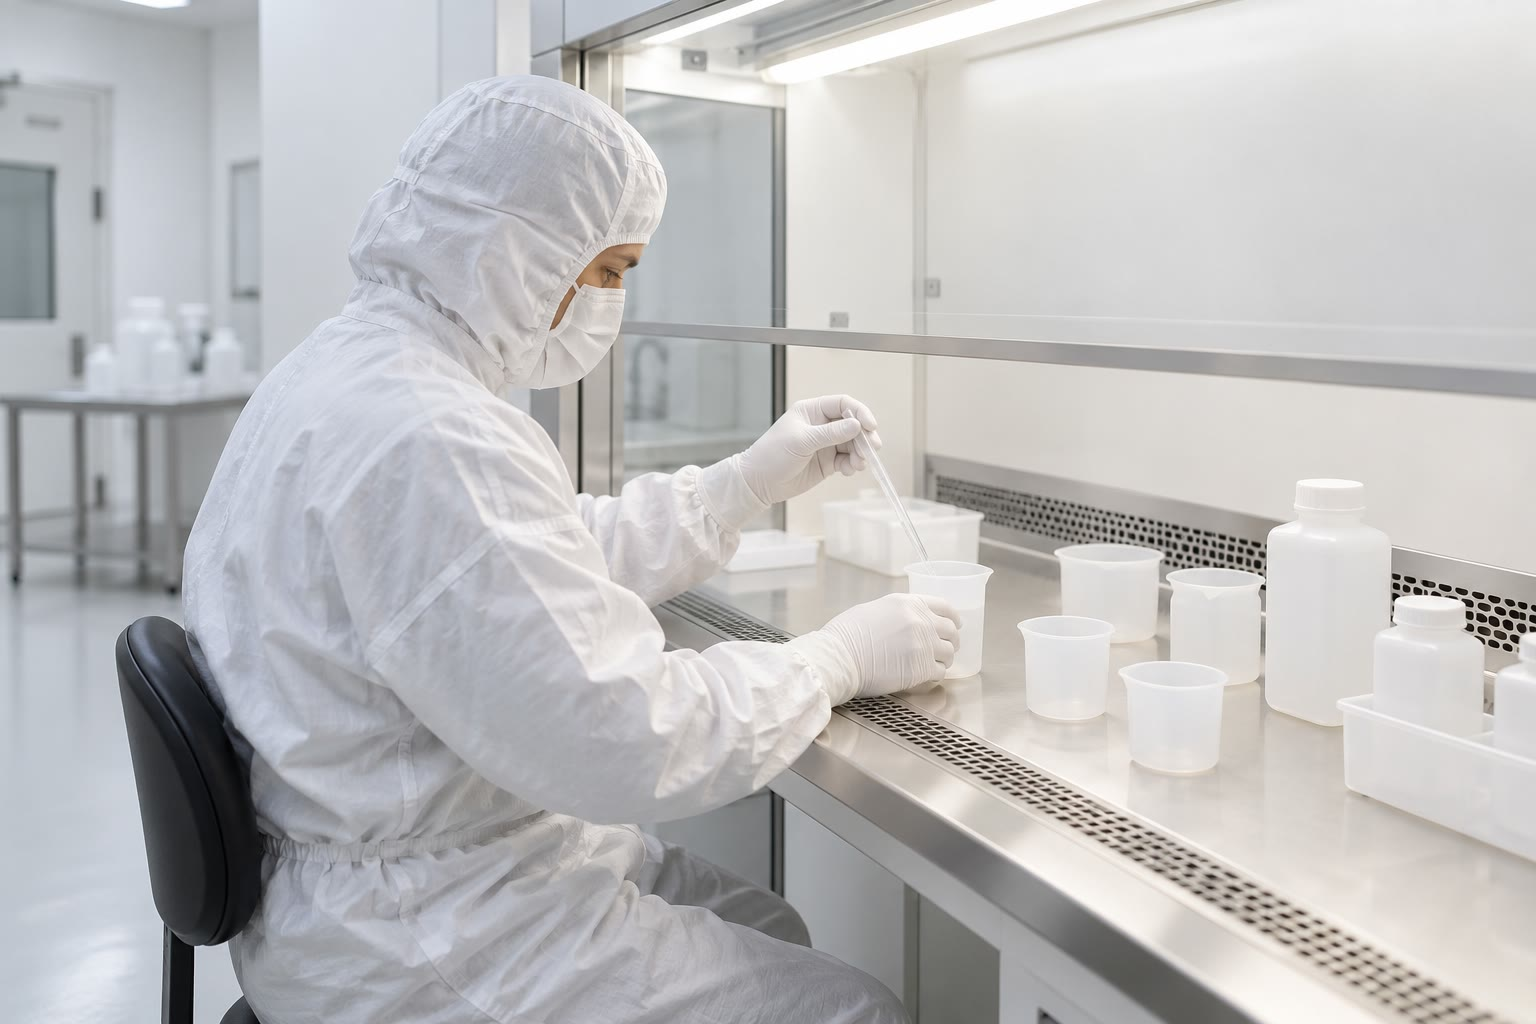
\includegraphics[width=\linewidth]{images/book4/ai/b2-clean-lab.jpg}

\smallskip
{\footnotesize A worker in a clean-room suit at the laminar-flow bench of a
geochemistry clean laboratory (AI-generated illustration).\par}
\end{minipage}
\end{inthelab}
% ledger: usgs:bhvo2-trace, usgs:bhvo2-origin

\section{Exercises}

\begin{exercise}[$\star$]\label{exo:b2:elements-in-the-earth:1}
The basalt BHVO-2 holds 0.5130 per cent \ce{K2O} and 2.731 per cent \ce{TiO2}
by mass. With the atomic masses K 39.10, Ti 47.87 and O 16.00, compute its
potassium and titanium contents in ppm.
\end{exercise}

\begin{exercise}[$\star$]\label{exo:b2:elements-in-the-earth:2}
In the \omterm{def:b2:elements-in-the-earth:bse}{bulk silicate Earth}, the ratios $(X/\mathrm{Mg})$ divided by the CI ratios
are 1.16 for aluminium, 0.22 for sodium, 0.077 for nickel and 0.0029 for
iridium. The \omterm{def:b2:planet-formation-meteorites:condensation}{condensation temperatures} of these elements are 1653, 958, 1353
and \qty{1603}{K}. Give the Goldschmidt class of each element and explain each
depletion.
\end{exercise}

\begin{exercise}[$\star$]\label{exo:b2:elements-in-the-earth:3}
The upper continental crust holds \qty{31}{ppm} of lanthanum and \qty{2.0}{ppm}
of ytterbium; \omterm{def:b2:elements-in-the-earth:ci}{CI chondrites} 0.232 and \qty{0.163}{ppm}. Compute the
chondrite-normalised values and $(\mathrm{La}/\mathrm{Yb})_N$. What does the
ratio say about the crust?
\end{exercise}

\begin{exercise}[$\star$]\label{exo:b2:elements-in-the-earth:4}
The upper continental crust holds 4.7, 1.0 and \qty{4.0}{ppm} of samarium,
europium and gadolinium; \omterm{def:b2:elements-in-the-earth:ci}{CI chondrites} 0.145, 0.0546 and \qty{0.198}{ppm}.
Compute $\mathrm{Eu}/\mathrm{Eu}^*$. Which mineral explains the result?
\end{exercise}

\begin{exercise}[$\star\star$]\label{exo:b2:elements-in-the-earth:5}
A garnet pyroxenite is made of 65 per cent clinopyroxene, 18 per cent garnet and
17 per cent olivine, orthopyroxene and spinel. The partition coefficients of
lanthanum are 0.058, 0.001 and 0.001, those of lutetium 0.53, 5.8 and 0.18.
Compute the bulk coefficients. Which element is compatible in the rock? Which
mineral holds most of the rock's lutetium?
\end{exercise}

\begin{exercise}[$\star\star$]\label{exo:b2:elements-in-the-earth:6}
The \omterm{def:b2:elements-in-the-earth:bse}{bulk silicate Earth} holds 22.8 per cent magnesium, \qty{2670}{ppm} of
sodium and \qty{1960}{ppm} of nickel; \omterm{def:b2:elements-in-the-earth:ci}{CI chondrites} 9.587 per cent,
\qty{5010}{ppm} and \qty{10640}{ppm}. Compute the Mg-normalised ratios to CI for
sodium and nickel. Both elements condense near \qty{1000}{K} or above; why is
nickel the more depleted?
\end{exercise}

\begin{exercise}[$\star\star$]\label{exo:b2:elements-in-the-earth:7}
A clinopyroxene crystallises from a melt with the composition of the mean MORB,
\qty{5.21}{ppm} of lanthanum and \qty{0.53}{ppm} of lutetium. Its partition
coefficients are 0.058 for lanthanum and 0.53 for lutetium. Compute its
lanthanum and lutetium contents, and the ratio of $(\mathrm{La}/\mathrm{Lu})_N$
in the crystal to that in the melt (CI: La 0.232, Lu \qty{0.0237}{ppm}).
\end{exercise}

\begin{exercise}[$\star\star$]\label{exo:b2:elements-in-the-earth:8}
Normalised to the \omterm{def:b2:elements-in-the-earth:bse}{primitive mantle} (Nb \qty{0.658}{ppm}, La \qty{0.648}{ppm}),
compute $(\mathrm{Nb}/\mathrm{La})_N$ for the upper continental crust (Nb 12,
La \qty{31}{ppm}), the Hawaiian basalt (18.10, \qty{15.20}{ppm}) and the mean MORB
(5.24, \qty{5.21}{ppm}). Which of them carries the signature of subduction zones?
\end{exercise}

\begin{exercise}[$\star\star$]\label{exo:b2:elements-in-the-earth:9}
Potassium and uranium are both highly incompatible. Compute the mass ratio K/U in
the \omterm{def:b2:elements-in-the-earth:bse}{primitive mantle} (K \qty{240}{ppm}, U \qty{0.0203}{ppm}), in the mean MORB
(\qty{0.160}{\percent} \ce{K2O}, U \qty{0.119}{ppm}) and in the upper continental
crust (\qty{2.80}{\percent} \ce{K2O}, U \qty{2.7}{ppm}), using
$\mathrm{K}/\ce{K2O} = 0.830$ by mass. What does the near-constancy of the ratio
mean, and why is K/U useful to estimate the potassium of a planet?
\end{exercise}

\begin{exercise}[$\star\star\star$]\label{exo:b2:elements-in-the-earth:10}
A small amount of melt is in equilibrium with the garnet pyroxenite of exercise
5. Show that, for two elements, the ratio
$(C_1/C_2)_{\mathrm{melt}}/(C_1/C_2)_{\mathrm{rock}}$ equals
$\bar D_2/\bar D_1$. Compute it for lanthanum and lutetium, and explain why the
melts of garnet-bearing mantle have steep rare earth patterns.
\end{exercise}

\begin{exercise}[$\star\star\star$]\label{exo:b2:elements-in-the-earth:11}
A mean MORB (Th \qty{0.404}{ppm}, Nb \qty{5.24}{ppm}) assimilates upper
continental crust (Th \qty{10.5}{ppm}, Nb \qty{12}{ppm}): a mass fraction $f$ of
crust mixes with $1-f$ of basalt. Show that the concentrations of the mixture are
linear in $f$ but that its ratio Th/Nb is not. Find $f$ for which Th/Nb reaches
0.2, and the ratio for $f = 0.1$.
\end{exercise}

\begin{exercise}[$\star\star\star$]\label{exo:b2:elements-in-the-earth:12}
Removing water, carbon or a metal core that contains neither aluminium nor
magnesium does not change the ratio Al/Mg of the rest: show it. In the \omterm{def:b2:elements-in-the-earth:bse}{bulk
silicate Earth}, $(\mathrm{Al}/\mathrm{Mg})$ is 1.16 times the CI value. If the
Earth kept all its aluminium, what fraction of its chondritic magnesium is
missing from the silicate Earth? With the Mg-normalised ratio of silicon,
0.83, what fraction of its chondritic silicon would be missing on the same
assumption?
\end{exercise}

\section{Problem: Weighing the core with a chondrite}

\begin{problem}[{Weekend problem --- reconstructing the bulk Earth from CI
chondrites, the mantle and the core, and weighing the core}]
\label{pb:b2:elements-in-the-earth:1}
A planetary geochemist wants to weigh the Earth's core without seismology, from
chemistry alone. She takes \omterm{def:b2:elements-in-the-earth:ci}{CI chondrites} as the starting material (Mg
\qty{95870}{ppm}, Al 8500, Si \num{106500}, Fe \num{182800}, Ni
\qty{10640}{ppm}), the \omterm{def:b2:elements-in-the-earth:bse}{primitive mantle} for the silicate Earth (MgO 37.8, FeO
8.05, NiO 0.25 per cent; Mg 22.8, Si 21.0 per cent), and a model core of 85.5
per cent Fe, 5.2 per cent Ni and 6.0 per cent Si. Atomic masses: Mg 24.31,
Si 28.09, Fe 55.85, Ni 58.69, O 16.00. Mass of the Earth
\qty{5.972e24}{kg}.

\medskip\noindent\textbf{Part I --- The chondritic starting point.}
\begin{enumerate}
\item Compute the mass ratios Fe/Mg, Ni/Mg, Si/Mg and Al/Mg of \omterm{def:b2:elements-in-the-earth:ci}{CI chondrites}.
\item Convert Fe/Si to an atomic ratio. Spectroscopy of the solar photosphere
gives 0.81 iron atom per silicon atom: is the comparison sensible?
\item \omterm{def:b2:elements-in-the-earth:ci}{CI chondrites} hold 2.1 per cent hydrogen and 3.5 per cent carbon, bound in
water-bearing minerals and organic compounds that the Earth did not keep. Why
do the ratios of question 1 not need correcting for this loss?
\item Why is magnesium a suitable reference element for the core problem, and
why could iron not serve?
\item Nickel, magnesium, iron and silicon condense within \qty{50}{K} of one
another (1353, 1336, 1334 and \qty{1310}{K}). Why does this support the
assumption that the bulk Earth kept their chondritic ratios? Which ratio of
question 1 departs from this group, and what does the chapter say about it?
\end{enumerate}

\noindent\textbf{Part II --- The silicate Earth.}
\begin{enumerate}[resume]
\item Convert the FeO and NiO of the \omterm{def:b2:elements-in-the-earth:bse}{primitive mantle} into Fe and Ni.
\item Compute Fe/Mg and Ni/Mg in the silicate Earth.
\item What fraction of the chondritic Fe and Ni is missing from the silicate
Earth, at constant magnesium?
\item The same calculation for iridium (\omterm{def:b2:elements-in-the-earth:bse}{primitive mantle} \qty{3.2}{ppb}, CI
\qty{0.470}{ppm}) gives a missing fraction of 99.7 per cent. Why is it larger
than for nickel, and nickel's than for iron?
\item Where is iron in the silicate Earth, and why did all of it not go to the
core?
\end{enumerate}

\noindent\textbf{Part III --- Weighing the core.}
\begin{enumerate}[resume]
\item Write the iron balance of the Earth with the core mass fraction $x$, and
derive \cref{prop:b2:elements-in-the-earth:core}.
\item Compute $y = x/(1-x)$ and $x$ from iron.
\item Do the same from nickel.
\item The two estimates do not agree exactly. Combine them by least squares:
minimise $\sum (a_iy - b_i)^2$, where $a_i y = b_i$ are the two equations of
questions 12 and 13, and give the best $y$ and $x$.
\item Why does the least-squares value lie so close to the iron estimate?
\item From the two equations, compute the Fe/Ni ratio of the core that would make
both exact. Compare with the model core.
\item Give the mass of the core.
\end{enumerate}

\noindent\textbf{Part IV --- Checks and consequences.}
\begin{enumerate}[resume]
\item Seismology gives a core of 32.5 per cent of the Earth's mass. By how many
per cent does the chemical estimate differ?
\item With a core of 32.5 per cent, how much iron would the core need to hold to
close the iron balance? Is this compatible with a core that is 10 per cent light
elements?
\item The model core holds 9.3 per cent of elements other than Fe and Ni. Which
light elements are candidates, and what evidence in the chapter supports silicon?
\item Compute, with $y$ of question 14, the silicon content of the core that would
make the bulk Earth's Si/Mg chondritic.
\item Compare with the model's 6 per cent. Suggest a reason, from the previous
chapter, why some silicon might be missing from the Earth altogether.
\item The model core holds \qty{0.5}{ppm} of gold, the \omterm{def:b2:elements-in-the-earth:bse}{primitive mantle}
\qty{1}{ppb}. With a core of 32.5 per cent, what fraction of the Earth's gold is
in the core?
\item State the core mass fraction of the Earth obtained from chemistry alone,
the key number of this problem.
\end{enumerate}
\end{problem}
% ledger: lodders:ci-table, lodders:ci-h-photo, ms95:pm-oxides, ms95:pm-trace, mcd03:core, earth:mass, badro:core, lodders:tc-table
